\chapter{Avoiding brute force}
\label{chap:approx}

\section{Method}

The grid search we talked about previously is both slow and not intellectually satisfying. Thus we looked for a smarter alternative that would reduce the number of call to the distance function while still finding low distance regions, possibly in agreement with the ground truth.

The basic idea is rather simple. The EMD distance is zero when all the points one of side share their positions with points in the other side. On the other hand, when one point is far away from all the others, we have to move it there and it is expensive. Therefore we want to reduce the search space by preprocessing all venues in the target city and keeping on the one close to the venues in the query region. To see why it may work, consider \autoref{fig:pigalle_barca}. If we restrict ourselves to the 100 nearest neighbors of each venues in the query region, we recover most of the ground truth venues (here we mean neighbors in the mathematical sense, so that for a venue $v$, $N_k(v)$ is the set of the $k$ closest venues in the target city according to the ground metric between individual venues).

\begin{figure}[b]
    \centering
    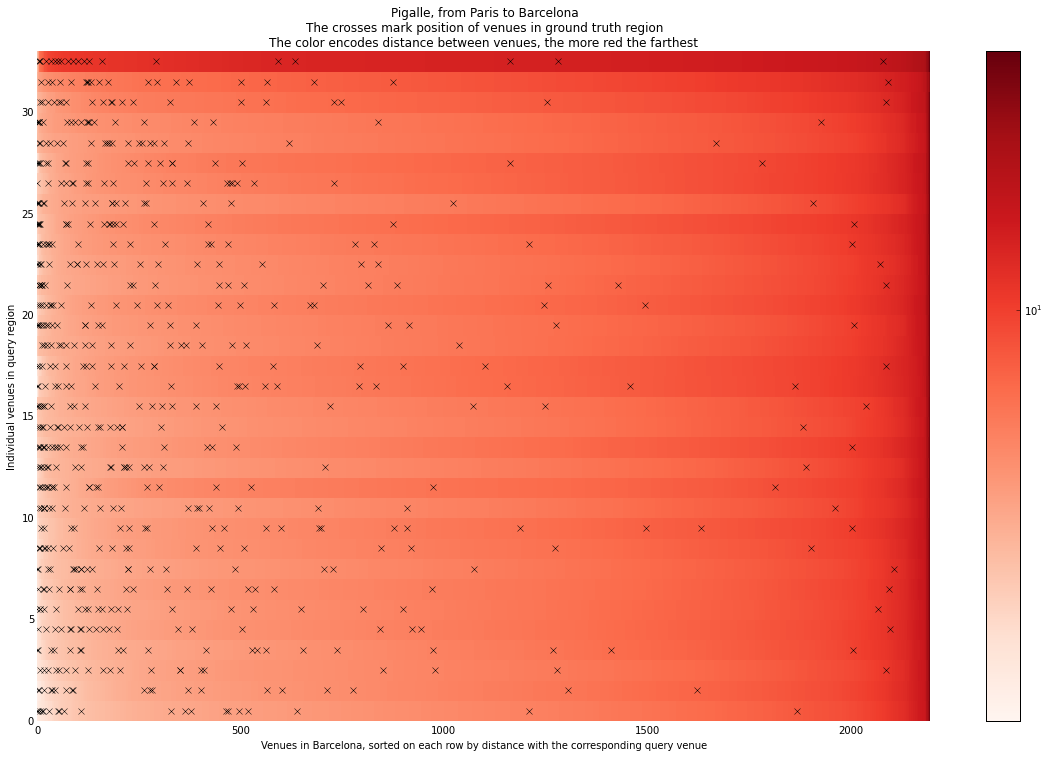
\includegraphics[width=1\linewidth]{pigalle_barca}
    \caption{The venues in ground truth area (black crosses) are mostly close from venues in the Paris query region (on the left).}
    \label{fig:pigalle_barca}
\end{figure}

The natural question arising is what the value of $k$ should be. The larger $k$, the more venues we retrieved, especially the more gold venues. But it also make the search space larger, because it covers a larger proportion of the city. This trade off is visualized in \autoref{fig:coverage_recall}, where each points of each query is obtained for a value of $k$ ranging from $1$ to $256$. We chose $k=50$ because in most cases, it returns 50\% of the gold venues while covering 33\% of the city in average. These number hint that the precision is rather low and we need another step to further reduce the search space.

\begin{figure}[tb]
    \centering
    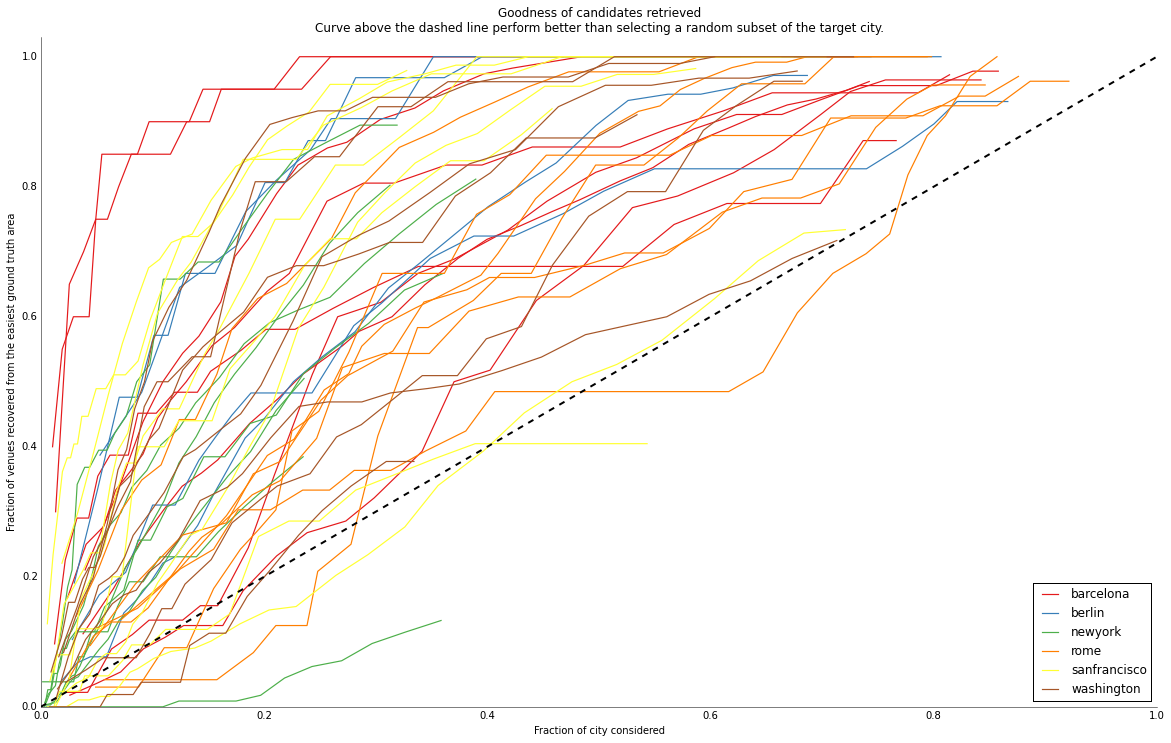
\includegraphics[width=1\linewidth]{coverage_recall}
    \caption{.}
    \label{fig:coverage_recall}
\end{figure}

There are many candidates but because we are looking for neighborhood, we can discard those in low density area. We run DBSCAN with a initial set of parameters. Depending of the results we recurse over larges cluster with stricter parameters or over the whole city with more flexible ones until enough cluster candidate of sensible size. We transform them into region and compute EMD.

\section{Results}
\subsection{How good it approximates grid EMD}

The full results \autoref{fig:approx_ratio} and the time ratio \autoref{fig:approx_time}. Can be presented as boxplot \autoref{fig:approx_box}, especially if we vary a discrete parameters: how many time we dilate the original convex hull. We expect that in some case, it could yield region with smaller distance. But in any case, it will take more time because there are more EMD computations to do (maybe we can prune some regions because initially there are very far from the best one we had so far and thus expanding them make little sense).

\begin{figure}[h]
    \begin{subfigure}[b]{\textwidth}
        \centering
        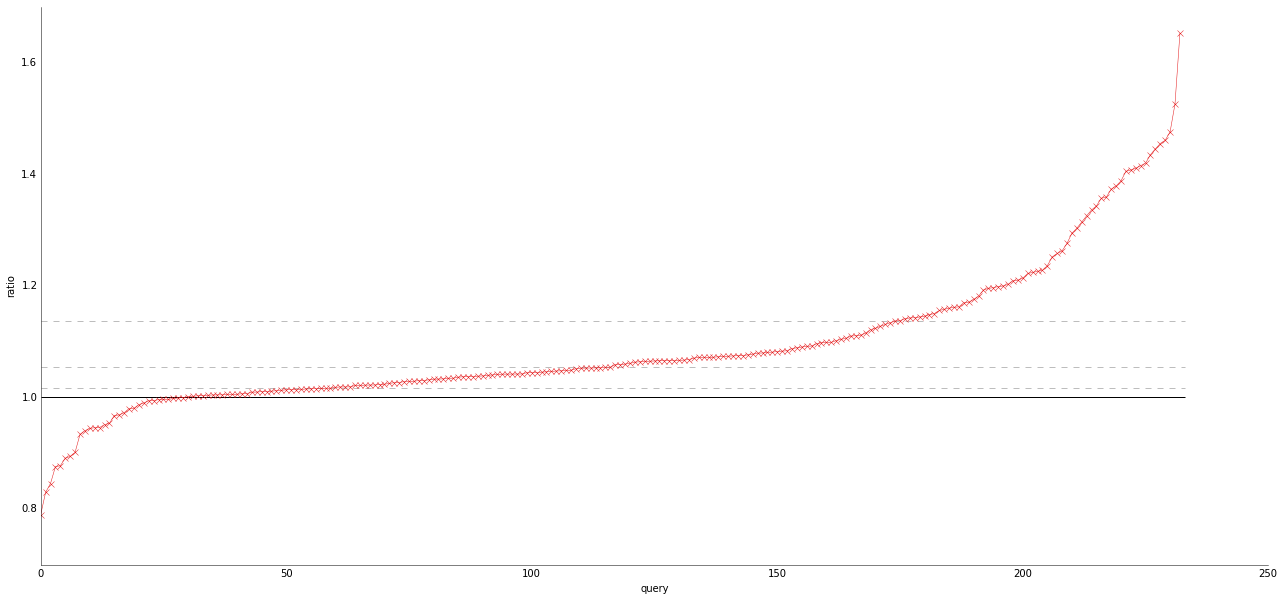
\includegraphics[width=\linewidth]{approx_ratio}
        \caption{Approximation ratio}
        \label{fig:approx_ratio}
    \end{subfigure}

    \begin{subfigure}[b]{\textwidth}
        \centering
        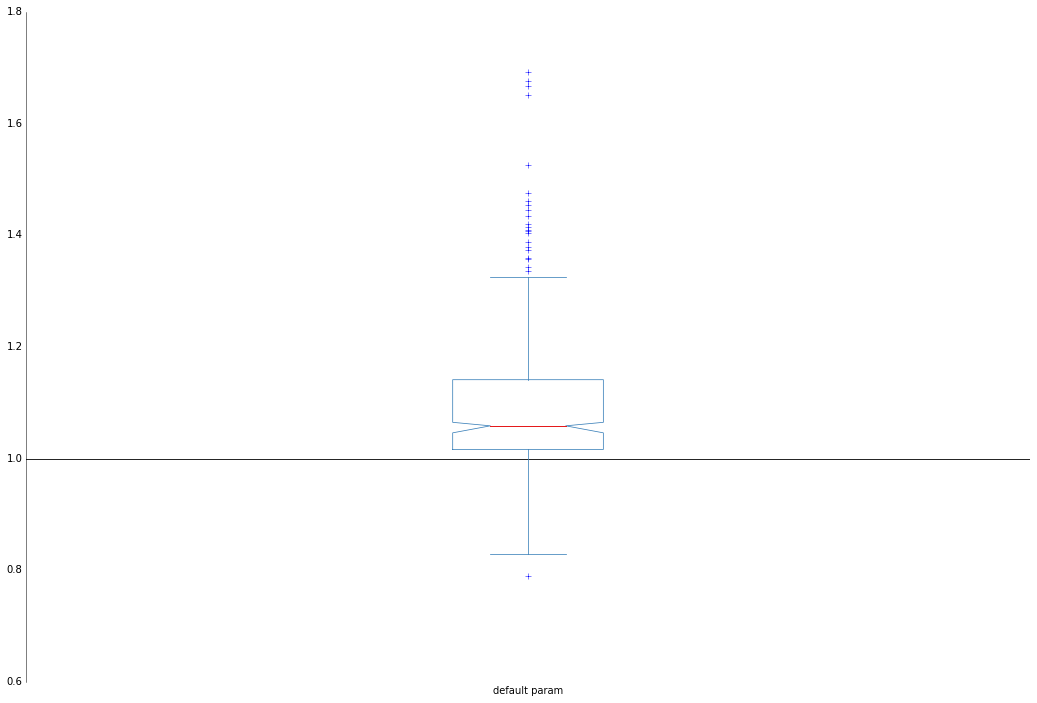
\includegraphics[width=\linewidth]{approx_box}
        \caption{The same data as a notched box plot.}
        \label{fig:approx_box}
    \end{subfigure}

    \begin{subfigure}[b]{\textwidth}
        \centering
        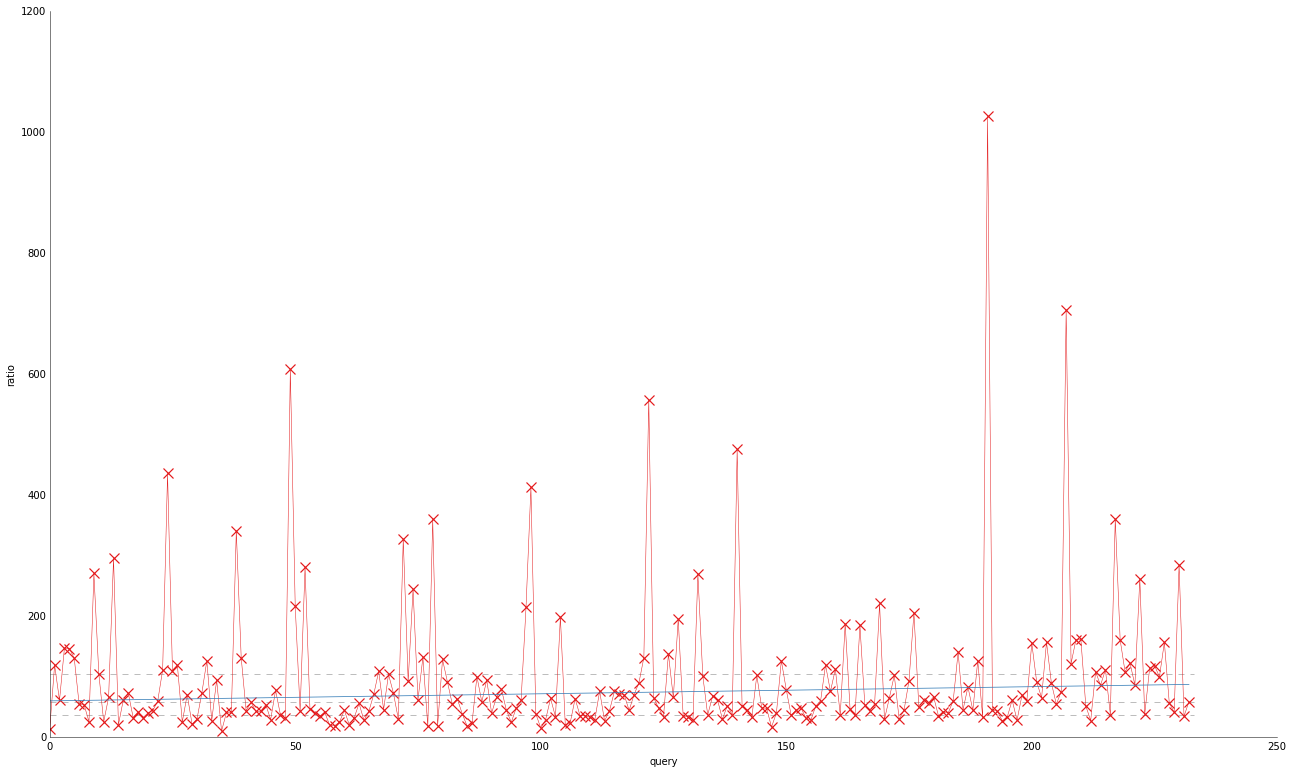
\includegraphics[width=\linewidth]{approx_time}
        \caption{How many times approximation method is faster than brute force.}
        \label{fig:approx_time}
    \end{subfigure}
    \caption{Approximation of grid EMD}
\end{figure}

\subsection{How well it matches ground truth}

There are two reason why it fails:
\begin{itemize}
    \item there are too few close neighbors in the ground truth region to form a cluster. Since it was the main assumption, we are screwed.
    \item There is cluster in the ground region but some clusters elsewhere have smaller EMD distance. In that case, it's a failure of EMD to recognize gold region of not of the approximation itself (although it would be nice to find a way to avoid those cases).
\end{itemize}
